\documentclass[runningheads,a4paper]{llncs}
\usepackage{amssymb}
\usepackage{url}
\usepackage{times}
\usepackage{float}
\usepackage[T1]{fontenc}
\usepackage{graphicx}
\usepackage{color}
\usepackage{soul}  
\usepackage{nameref}  
\usepackage{amsbsy}  
\usepackage{bezier}  
\usepackage{colortbl}  
\usepackage[leqno,fleqn]{amsmath}  
\usepackage{verbatim}
\usepackage{listings}
\usepackage{qtree}
\usepackage{float}
\floatstyle{boxed}
\restylefloat{figure}
\usepackage{cite}
% deutsche Silbentrennung
\usepackage[ngerman]{babel}
% wegen deutschen Umlauten
\usepackage[utf8]{inputenc}

\setcounter{tocdepth}{3}
\newcommand{\keywords}[1]{\par\addvspace\baselineskip
\noindent\keywordname\enspace\ignorespaces#1}

\begin{document}
\mainmatter

\title{Software Projekt Anwendungen von Algorithmen}
\subtitle{Metaheuristiken II}
\date{Wintersemester 2014/2015}

\author{Robert Lion Gottwald, Lars Parmakerli, Phil Schmidt}

\institute{
Freie Universit\"at Berlin\\ Institut for Computer Science \\ robert.gottwald@fu-berlin.de \\ -Lars - fu-Adresse-\\  philschmidt@inf.fu-berlin.de \\
\url{https://www.inf.fu-berlin.de/lehre/WS14/SWPAlg/index.html}
}
\maketitle
\begin{abstract}
Der folgende Text befasst sich mit der Arbeit der Gruppe Metaheuristiken II des Softwareprojekts Anwendungen von Algorithmen im Wintersemester 2014/15. Dabei werden wir uns mit zwei  spezifischen Metaheuristiken befassen, namentlich Simulated Annealing und ein genetisch-inspiriertes Verfahren, sowie mit dem globalen Lösungsverfahren Branch-and-Bound und seinen Schwierigkeiten für die Anwendung auf unsere Probleme und schließlich zuletzt mit nicht-linearen Optimierungsverfahren unter Zuhilfenahme numerischer Verfahren bezogen auf die gewählten Aufgabenstellungen de Stapelns und des Packens.

\end{abstract}

\section{Metaheuristiken}

Das Wort Metaheuristik setzt sich aus den beiden wörtern 'Meta' und 'Heuristik'  zusammen.
Eine Heuristik ist ein Verfahren, welches für eine bestimmte Art von Problemen eine Lösung findet, die als ausreichend 'gut' erachtet wird. 
Das Wort 'Meta-' bedeutet in diesem Kontext 'auf einer Höheren Ebene'.

Eine Metaheuristik ist demnach möglichst effizientes Lösungsverfahren, welches sich auf einer höher abstahierten Ebene abspielt und somit kein Wissen über das unterliegende Problem benötigt. Die einzige bestehende Voraussetzung für das Anwenden einer Metaheuristik auf ein System, ist eine Funktion existiert, welche die Güte einer Lösung berechnen kann.

Metaheuristiken stellen nützliche Werkzeuge dar, um Optimierungsproleme in komplexeren Systemen zu lösen, ohne für diese eine spezifische, kompliziertere Heuristik zu entwerfen, sind also sozusagen wiederverwendbare Lösungswege. Der Nachteil von Metaheuristiken liegt in der Effizienz in Laufzeit, sowie der meist niedrigeren Güte der erzielten Lösung.

In unserem Softwareprojekt bestehen Metaheuristikmodule aus generischen Klassen mit einem Typenparameter für die Anwendungsdomäne, sowie mindestens einer Auswertungsfunktion. Einzelne Implementierungen werden in den Folgekapiteln beschrieben.


\section{Simulated Annealing}

\subsection{Inspiration}

Metaheuristiken liegen zumeist realen Prozessen zugrunde, welche ein bestimmtes verhalten aufweisen. Simulated Annealing ist vom namensgebenden Annealing-Prozess aus der Schwerindustrie inspiriert.

Beim Annealing wird Metal Metall stark erhitzt und über einen längeren Zeitraum langsam abgekühlt. Bei den hohen Temperaturen tritt eine starke Molekular-Bewegung im zu bearbeitenden Material auf. Dadurch, dass der Abkühlungsprozess über einen längeren Zeitraum gestreckt wird, reduziert sich die Teilchenbewegung auch nur allmählich. Der Abkühlungsprozess wird so gesteuert durch etwaige Behandlungsmethoden, dass die einzelnen Teilchen einen für einen bestimmten zu erzielenden Effekt, wie zum Beispiel eine stabile Statik, guten Zustand einnehmen.

Wie der Name uns sagt, ist die Herangehensweise beim Simulated Annealing nun so, dass wir einen derartigen physikalischen Prozess über einen abstrakten Wertebereich simulieren.

\subsection{Simulation}

Das zu behandelnde Metall wird in unserer Implementierung durch einen generischen Typ-Parameter namens 'State' realisiert. Bei der Anwendung auf die uns gegebene Problemstellung, wie zum Beispiel Stapeln, ist dies ein Feld aus Polygonen.

Die Molekularbewegung wird durch eine Umgebungsfunktion namentlich 'Mutator' umgesetzt. Eine Umgebungsfunktion Bekommt einen 'State' als Input und gibt einen anderen 'State' zurück, der in der 'Nachbarschaft' des Eingabe-States befindet.

Die benötigte Gütefunktion, die jedem 'State' einen Double-Wert zuweist und für jede Metaheuristik notwendig ist, ist als Quantifizierung des durch das Annealing zu erzielenden Effekts zu interpretieren.

Die Unberechenbarkeit des Materials, beziehungsweise das chaotische Verhalten der Teilchen, lässt sich durch die Temperatur messen. In unserer Simulation wird eine CoolingSchedule-Klasse verwendet, die nach beliebig wählbaren Abkühlmustern, wie zum Beispiel logarithmisches oder lineares Abkühlen, nach jedem Abfragen einer T()-Funktion eine neue Temperatur zurückgibt.

\subsection{Ablauf}

Simulated Annealing ist ein iteratives Verfahren. Wir nutzen zwei Zeiger; einen, der auf das aktuell beste gefundene Ergebnis zeigt ('best'), und einen, der den aktuellen Ist-Zustand der Domäne speichert ('current'). In jeder Iteration wird ein Neuer State in der Umgebung des aktuellen States mithilfe des Mutators generiert.

Anschließend wird die Objective Function dazu genutzt, den neuen State zu bewerten und mit den alten States zu vergleichen. Ist ein neues globales Optimum gefunden worden, wird dieses gespeichert (best).

Für die Bestimmung des neuen current-Zustandes wird eine zufällige Zahl zwischen 0 und der Maximaltemperatur generiert. Im Normalfall nimmt current den nach Gütefunktion besseren State an, es sei denn es wird ein kleinerer Wert, als die aktuelle Temperatur gewürfelt. Dann nimmt current den schlechteren der beiden Werte an.

Dieser Prozess wird solange fortgeführt, bis entweder eine feste Iterationsanzahl erreicht ist, oder die Lösung 'gut'-genug ist. Unsere Implementierung terminiert einfach nach einer Festen Schrittzahl.

\section{Genetische Heuristik}

\subsection{Inspiration}

Ähnlich wie beim Simulated Annealing gibt es für den folgenden genetischen Algorithmus Inspiration durch einen real-weltlichen Prozess. In diesem Fall ist es das biologische Konzept der Evolution.

Evolution wird ein biologischer Prozess genannt, der optimale Adaption von Lebensformen an einen bestimmten Lebensraum über mehrere Generationen erlaubt. Dieser Prozess lässt sich in verschiedene Iterationen (Generationen) aufteilen. Jede Iteration kennt verschiedene Phasen, die sie durchläuft, die den Evolutionsvorgang ausmachen:

\begin{description}
	\item[Natürliche Selektion] \hfill \\ Das Ökosystem um eine Population herum übt einen so genanten Selektionsdruck auf die darin lebenden Organismen aus. Lebensformen, die nicht bestimmten Ansprüchen genügen, werden aus dem Genpool eliminiert.

	\item[Rekombination] \hfill \\ Durch sexuelle Fortpflanzung wird es zwei genetisch 'fit'-en Organismen ermöglicht, ihre Gene untereinander auszutauschen. In der nächsten Generation werden ihre Nachkommen eine zufällige Auswahl an Genen ihrer beiden Elternteile tragen.

	\item[Mutation] \hfill \\ Im Vorgang der Gen-Rekombination kann es vorkommen, dass Reproduktions-Fehler auftreten. Die Folge davon ist, dass die nachkommen Gen-Eigenschaften haben können, die nicht Teil des ursprünglichen Genpools der Elterngeneration waren. Diese Mutationen treten zufällig auf und haben ebenso willkürliche Auswirkungen.
\end{description}

Nachdem durch diesen Prozess eine neue Generation erschaffen wurde, durchläuft diese Generation erneut den selben Prozess. Dabei verbessert sich langfristig das Gen-Material in Bezug auf den Selektionsdruck des bestehenden Ökosystems. Der folgende Algorithmus versucht sich daran,  ein derartiges Ökosystem mit verschiedenen Populationen zu simulieren, um einen ähnlichen Optimierungsprozess zu erzielen.

\subsection{Simulation}

Ein individuelles Mitglied einer Population (Individuum), wird in unserer Implementierung durch einen generischen Typ-Parameter namens 'State' realisiert. (Der im Bezug auf das biologische Konzept nicht ganz aussagekräftige Name 'State' ist an dieser Stelle der einheitlichen Gestaltung der Schnittstellen für die verschiedenen Metaheuristiken geschuldet) Im Zusammenhang mit unserem Algorithmus steht ein solches Individuum für eine (potentiell befriedigende) Lösung des gegebenen Problems. Angewendet auf das Stapel-Problem wäre das beispielsweise eine bestimmte Anordnung von Polygonen.

Die Natürliche Selektion wird in unserem Algorithmus mit Hilfe von Instanzen des generischen 'Survival'-Typs simuliert. Das entsprichende Interface spezifiziert die 'findSurvivors'-Methode, die, ausgehend von der konkreten Implementierung, aus der aktuellen Population diejenigen Individuen auswählt, die schließlich die neue Generation bilden. Ein naheliegender Ansatz für die Implementierung wäre beispielsweise ein Verfahren, das die n fittesten Individuen (also die n aktuell besten Lösungen für das Problem) auswählt. Eine weitere beliebte Möglichkeit stellen randomisierte Auswahlverfahren dar.

Die Berechnung der Güte eines konkreten Individuums erfolgt mit Hilfe einer Bewertungsfunktion, die über das Interface 'ObjectiveFunction' definiert werden kann. Für das Packen und Stapeln entspricht das beispielsweise der Berechnung der Fläche der konvexen Hülle.

Für die Rekombination steht in unserer Implementierung das 'CrossOver'-Interface zur Verfügung. Hier wird die 'cross'-Methode spezifiziert, die als Parameter Individuen aus der aktuellen Population entgegennimmt und neue zurückgibt. An dieser Stelle abstrahieren wir von dem biologischen Konzept, indem wir nicht nur Rekombinationen von zwei Elternteilen zulassen. Die Methode erhält als stattdessen eine beliebig lange Liste von Individuen und kann ebenso eine beliebig lange Liste von neu kombinierten Individuen zurückgeben.     

Das Konzept der Mutation wird durch das 'Mutator'-Interface bereitgestellt. Dies spezifiziert die 'mutate'-Methode, welche aus einem als Parameter übergebenen Mitglied der Population ein neues (mutiertes) Individuum erzeugt. Als konkrete Implementierung für das Packen-Problem ist beispielsweise randomisiertes Verschieben und Drehen der einzelnen Polygone möglich oder ein Verschieben bis zum nächsten Schnittpunkt mit einem anderen Polygon.

\subsection{Ablauf}

Dem Konstruktor der 'GeneticAlgorithm'-Klasse werden zunächst folgende Parameter übergeben:
\begin{enumerate}
\item Die gewünschte Größe einer Population 
\item Die gewünschte Anzahl an Iterationen (Eine Iteration entspricht der Herausbildung einer neuen Generation)
\item Die Anzahl der mutierten und rekombinierten Individuen für jede Iteration
\item Die 'Survival'-, 'CrossOver'-, 'ObjectiveFunction' und 'Mutator'-Objekte
\end{enumerate}
Aus einem initial gegeben 'State' wird zunächst mit Hilfe von Mutationen die Ausgangspopulation erstellt. Das beste Individuum wird als aktuell beste Lösung gespeichert. Anschließend werden iterativ neue Generationen herausgebildet, wobei durch Mutation und Rekombination solange neue Individuen zu der aktuellen Population hinzugefügt werden bis die spezifizierte Anzahl erreicht ist. Anschließend wird durch das 'Survival'-Objekt die neue Generation ausgewählt. Nach jeder Iteration wird erneut ermittelt ob ein besseres Individuum, als das aktuell beste erzeugt wurde. Nachdem die festgelegte Anzahl von Iterationen durchlaufen wurde wird das die beste Lösung zurückgegeben. 

\section{Branch and Bound}

Branch and Bound ist ein Entwurfsmuster für Lösungsalgorithmen von Optimierungsproblemen. Unserer Gruppe wurde von Veranstalterseite empfohlen, uns mit diesem System zu befassen und  die Möglichkeiten, einer Anwendung der Branch and Bound Methode zur Konstruktion eines Algorithmus für die Bearbeitung des Stapel- oder Packen-Problems, einzuschätzen.

In den folgenden beiden Abschnitten werden wir das generelle Entwurfsschema Branch and Bound erläutern und seine Tauglichkeit für die Behandlung der Problemstellungen des Projekts evaluieren.

\subsection{Das Verfahren}

Branch and Bound basiert auf einer selektiven Suche durch bestimmte, gewählte Teilmengen der Menge aller möglichen Belegungen. Das Vorgehen besteht aus den zwei namensgebenden Schritten Branch und Bound.

Im Branch-Schritt wird ein Lösungsbaum generiert, in dem iterativ das Problem mit jedem Schritt in immer weiter vereinfachte Teilprobleme aufgeteilt wird. Zur Veranschaulichung: Eine der einfachsten Vereinfachungen wäre es, einen Parameter auf einen fixen Wert festzulegen, oder auf einen bestimmten Wertebereich einzugrenzen. 
Dadurch entsteht ein möglicherweise sehr großer Baum, der alle möglichen Parameterbelegungen hierarchisch ordnet.

Der Bound-Schritt entfernt nun Teilprobleme, deren mögliche Lösungen nicht ausreichend gut sind. Für jedes Teilproblem wird zu diesem Zwecke eine obere und eine untere Schranke berechnet. Dazu können beispielsweise Heuristiken oder spezifische Kennwerte des Problems herangezogen werden.
Sollten nun bei einem Minimierungsproblem, wie unserem, Teilprobleme/Zweige mit einer unteren Schranke gefunden werden, die größer als die obere Schranke eines anderen Teilproblems, so brauchen wir in diesem Zweig nicht weiter nach einer Lösung suchen. Der Zweig wird dann entsprechend vom Baum abgetrennt und nicht weiter aufgefächert.

\subsection{Tauglichkeit}

Branch and Bound lässt sich theoretisch auf jede Art von Problem anwenden, jedoch stellt sich stets die Frage, ob für eine Zerlegung Schranken gefunden werden können, die scharf genug sind, um die Suche auf eine Teilmenge einzuschränken, die klein genug ist. 
Findet sich das nicht, entartet Branch and Bound zu einer einfachen brute-force Suche durch den Lösungsraum nach einer guten Lösung.

--------------------TODO-------------------------

\section{Nicht-lineare Optimierung mit numerischen Verfahren des Stapelproblems}

\subsection{Formulierung als nicht-lineares Optimierungsproblem}
\label{formObjStacking}
Das Stapelproblem lässt sich als Optimierungsproblem einer nicht-linearen Zielfunktion ohne Nebenbedingungen formulieren. Die Zielfunktion ${f: \mathbb{R}^n \rightarrow \mathbb{R}}$ erhält die Translations-Vektoren und die Rotationswinkel für jedes der gegebenen Polygone als Eingabe und ordnet diesen die Fläche der konvexen Hülle, bzw. der Bounding-Box, zu. Im zweidimensionalen sind das also drei Parameter für jedes Polygon.

\subsection{Lösungs-Verfahren}
\label{sec:uncon_nonlin_opt}

\subsubsection{Newton-Verfahren}

Für derartige Optimierungsprobleme gibt es verschiedene mathematische Verfahren zur numerischen Berechnung lokaler Optima. Viele dieser Verfahren basieren auf dem Newton-Verfahren zum finden von Nullstellen einer Funktion. Um das Newton-Verfahren zur Optimierung einzusetzen, wendet man es auf die erste Ableitung $f'$ an. Wenn die Lösung dann zu einer Nullstelle konvergiert ist, ist die erste Ableitung null und damit ein Extrempunkt erreicht. Allerdings benötigt das Newton-Verfahren auch noch die erste Ableitung der Funktion auf die es angewendet wird, deshalb wird auch noch die zweite Ableitung $f''$ benötigt, wenn man das Newton-Verfahren zur Optimierung verwendet.

Das Verfahren berechnet die Lösung iterativ. Eine gegebene Lösung $x_n$ wird in jedem Schritt mit der Formel
\begin{equation*}
x_{n+1} = x_n - \frac{f'(x_n)}{f''(x_n)}
\end{equation*}
weiter der optimalen Lösung angenähert.

Bei der Minimierung der Funktion aus \ref{formObjStacking} ist die erste Ableitung eine vektorwertige Funktion, die einen Vektor mit partiellen Ableitungen, den Gradienten, zurückgibt ${f': \mathbb{R}^n \rightarrow \mathbb{R}^n}$ und die zweite Ableitung gibt dann sogar eine ${n\times n}$-Matrix zurück, nämlich die partielle Ableitung nach jedem der $n$ Eingabeparameter für jede der $n$ Komponenten des Ausgabevektors der ersten Ableitung ${f'': \mathbb{R}^n \rightarrow \mathbb{R}^{n\times n}}$. Diese Matrix wird Hesse-Matrix genannt.

Um das Newton Verfahren für vektorwertige Funktionen einzusetzen wird die Formel zu
\begin{equation}
\label{eq:ndimnewtonstep}
x_{n+1} = x_n - H^{-1}g
\end{equation}
Dabei ist $H := f''(x_n)$ die Hesse-Matrix und $g := f'(x_n)$ der Gradient.

Anstatt aber die Inverse direkt zu berechnen, ist es günstiger den Iterations-Schritt ${s_n := x_{n+1} - x_n}$ durch lösen des linearen Gleichungssystems
\begin{equation}
\label{eq:newtonlineq}
Hs_n=-g
\end{equation}
zu berechnen und dann ${x_{n+1} = x_n + s_n}$.


\subsubsection{Ableitungen}

Da wir in der Implementierung der Zielfunktion \ref{formObjStacking} die Ableitungen nicht gegeben haben, müssen wir sie numerisch approximieren. Mit der Finite-Differenzen-Methode benötigt die Berechnung der ersten Ableitung zwei Funktionsauswertungen pro Komponente, also insgesamt $2n$ Funktionsauswertungen. Würde man nun die zweite Ableitung $f''$ ebenfalls numerisch approximieren, bräuchte man $2n$ Auswertungen von $f'$, also insgesamt $4n^2$ Auswertungen der ursprünglichen Funktion $f$. Das ist nicht nur sehr aufwendig, sondern auch problematisch für die numerische Stabilität des Verfahrens. Denn die Finite-Differenzen-Methode führt leicht zu Auslöschungen, die bei der Subtraktion fast gleich großer Gleitkommazahlen auftreten.

Außerdem ist die Ableitung der Zielfunktion für das Stapelproblem nicht glatt, denn wenn ein Polygon sich komplett innerhalb der konvexen Hülle befindet, ist die Ableitung bezüglich dessen Translations- und Rotationsparameter null. Sobald das Polygon jedoch so weit verschoben wird, dass es den Rand erreicht, wird die Ableitung positiv, hat also an dieser Stelle einen knick und die zweite Ableitung ist somit nicht stetig. Beweise für die Konvergenzeigenschaften von Newton-artigen Verfahren setzten jedoch zweimal stetig differenzierbare Funktionen voraus.

In der Praxis hat sich jedoch gezeigt, dass es Newton-artige Verfahren zur Optimierung gibt, die gut für nicht-glatte Funktionen funktionieren \cite{DBLP:journals/mp/LewisO13} und ohne zweite Ableitungen auskommen.

\subsubsection{Quasi-Newton Verfahren}

Sogenannte Quasi-Newton Verfahren, sind Newton-artige Verfahren, die die direkte Berechnung der zweiten Ableitung vermeiden. Stattdessen wird eine Approximation der Hesse-Matrix verwaltet, die in jeder Iteration des Algorithmus mithilfe der Informationen der ersten Ableitung weiter der echten Hesse-Matrix angenähert wird. Dafür existieren verschiedene Update-Formeln. Wir verwenden die BFGS Update-Formel, benannt nach ihren Erfindern \textbf{B}royden, \textbf{F}letcher, \textbf{G}oldfarb und \textbf{S}hanno. \cite{nocedal1999numerical}
\begin{equation*}
B_n+1 = B_n + \frac{(y_n- B_ns_n) (y_n-B_ns_n)^T}{(y_n- B_n s_n)^T s_n}
\end{equation*}
wobei $B_n$ die Approximation der Hesse-Matrix in Schritt $n$ ist und
\begin{equation*}
s_n := x_{n+1} - x_n = -B_n^{-1}*g\\
y_k := f'(x_{n+1}) - f'(x_n)
\end{equation*}

Ausserdem gibt es noch eine Variante der Formel um direkt die Inverse Hesse-Matrix zu approximieren. Das hat den Vorteil, dass der Quasi-Newton-Schritt wie in Gleichung (\ref{eq:ndimnewtonstep}) berechnet werden kann und daher kein lineares Gleichungssystem in jedem Schritt gelöst werden muss wie in Gleichung (\ref{eq:newtonlineq}). Diese Variante verwenden wir auch in unserer Implementierung des BFGS-Verfahrens.
\begin{equation}
\label{eq:bfgsinverse}
B_{n+1}^{-1} = (I - p_n s_n y_n^T) B_n^{-1} (I - p_n y_n s_n^T) + p_n s_n s_n^T \\ p_n = \frac{1}{y_n^Ts_n}
\end{equation}

Die BFGS-Updateformel hat zusätzlich noch die Eigenschaft 

\subsubsection{Line search}

Für die globale Optimierung mit (Quasi-)Newton-Verfahren ist es oft nicht sinnvoll immer den vollen Schritt $s_n$ zu verwenden, sonder diesen zu skalieren. Die Schrittweite $\alpha$ soll so gewählt werden, dass der Funktionswert möglichst klein wird. Also die univariate Funktion
\begin{equation*}
\Phi(\alpha) = f(x_n + \alpha s_n)
\end{equation*}
minimal wird.

\begin{figure}[ht]
 \centering
 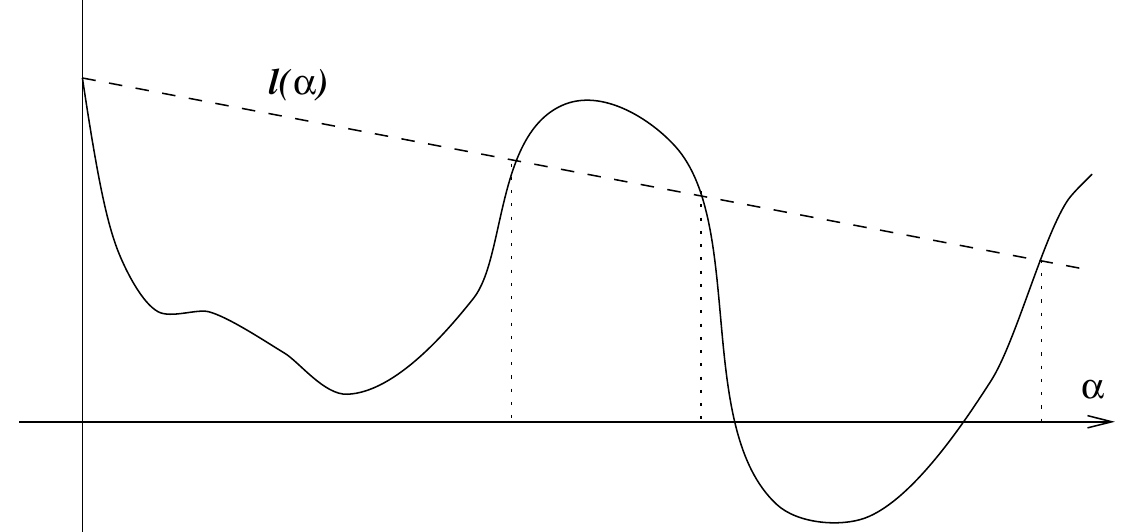
\includegraphics[scale=0.25]{armijo}
 \caption{Armijo Bedingung \cite{nocedal1999numerical}}
 \label{img:armijo}
\end{figure}

Dazu ist es wichtig, dass die Richtung $s_n$ eine Abstiegsrichtung ist, also der Funktionswert in dieser Richtung zunächst abnimmt. Das ist im Allgemeinen sehr aufwändig und es lohnt sich meistens nicht diesen Aufwand in jeder Iteration zu betreiben. Es reicht in der Praxis bestimmte Anforderungen an die gewählte Schrittweite zu stellen sodass die Konvergenz garantiert werden kann. Damit die Schrittweite nicht zu groß wird, wird häufig die Armijo-Bedingung verwendet.
\begin{equation}
\label{eq:armijo}
f(x_n+\alpha s_n) \le f(x_n)+c_1\alpha f'(x_n)^T s_n
\end{equation}
Dabei ist $f'(x_n)^T s_n = \Phi'(0)$ die Richtungsableitung von $f$ in Richtung $s_n$, welche negativ ist wenn $s_n$ eine Abstiegsrichtung ist. Die Bedingung erzwingt also, dass die Zielfunktion $f$ in Richtung $s_n$ proportional zur Steigung im Punkt $x_n$ und proportional zur Schrittweite abnimmt. Die Konstante $c_1 \in (0,1)$ kann frei gewählt werden, wobei kleinere Werte die Bedingung abschwächen.

Die gestrichelte Linie in Abbildung \ref{img:armijo} veranschaulicht die Armijo-Bedinung. Die Funktionswerte, die unter ihr liegen, erfüllen die Bedingung, die Funktionswerte darüber jedoch nicht. Die Armijo-Bedingung alleine reicht aber nicht um eine Kovergenz zu garantieren, denn ein genügend kleiner Schritt erfüllt die Bedingung immer. Dazu eignet sich die Krümmungs-Bedingung.
\begin{equation}
\label{eq:curvature}
f'(x_n+\alpha*s_n)^T s_n \ge c_2 f'(x_n)^T s_n
\end{equation}
Diese Bedingung erzwingt, dass die Funktion im gewählten Punkt nicht mehr so stark abnimmt wie im Punkt $x_n$. Wenn nämlich die Steigung in einem Punkt noch stark negativ ist, macht es Sinn noch weiter in diese Richtung zu gehen. Die Konstante ${c_2\in (c_1,1)}$ kann, wie $c_1$, frei gewählt werden, wobei kleinere Werte die Bedingung verstärken. Wir verwenden die Werte $c_1 = 1e-4$ und $c_2 = 0.9$, da sich durch experimentieren gezeigt hat, dass strengere Werte die Gesamtlaufzeit eher negativ beeinflussen.

\begin{figure}[ht]
 \centering
 \begin{description}
 \item[Eingabe] Startwert $x_0$, Zielfunktion $f$, maximale Iterationszahl $N$, Konstanten $c_1,c_2$.
 \item[Ausgabe] Eine bessere bzw. lokal optimale Lösung $x_{\text{\tiny{BFGS}}}$.
 \end{description}
 \begin{enumerate}
 	\item Wähle $u=0$, $v=\infty$ und $\alpha = 1$
 	\item Wiederhole:
 	\begin{enumerate}
 	\item Wenn Bedingung (\ref{eq:armijo}) für $\alpha$ verletzt ist, setze $v=\alpha$
 	\item Ansonsten wenn Bedingung (\ref{eq:curvature}) für $\alpha$ verletzt ist, setzte $u=\alpha$.
 	\item Ansonsten gebe $\alpha$ zurück.
 	\item Wenn $v < \infty$ setze $\alpha = \frac{u+v}{2}$
 	\item Ansonsten setze $\alpha = 2\alpha$
 	\end{enumerate}
 \end{enumerate}
 \caption{Line search Algorithmus \cite{DBLP:journals/mp/LewisO13}}
 \label{alg:linesearch}
\end{figure}

Die Bedingungen (\ref{eq:armijo}) und (\ref{eq:curvature}) zusammen nennt man die Wolfe-Bedingungen. Fügt man zur linken und rechten Seite der Bedingung (\ref{eq:curvature}) noch Beträge hinzu, dann spricht man von den starken Wolfe-Bedingungen. Wir verwenden jedoch die Variante ohne Berträge, denn die starken Wolfe-Bedingungen eignen sich nur für glatte Funktionen \cite{DBLP:journals/mp/LewisO13}.

Ein recht einfacher und für nicht-glatte Funktionen geeigneter Algorithmus um einen Punkt zu finden, welcher die Bedingungen (\ref{eq:armijo}) und (\ref{eq:curvature}) erfüllt, ist in Abbildung (\ref{alg:linesearch}) beschrieben. Beginnend mit der Schrittweite $\alpha=1$ verdoppelt er diese solange, bis ein Punkt gefunden wurde, der die Armijo-Bedingung verletzt. Dieser Wert für die Schrittweite wird dann als obere Schranke $v$ gesetzt. Daraufhin wird Bisektion verwendet, um im Intervall $(u,v)$ einen Punkt zu finden, der beide Bedingungen, (\ref{eq:armijo}) und (\ref{eq:curvature}), erfüllt. Immer wenn die Bedingung (\ref{eq:armijo}) verletzt ist, wird in der linken Intervallhälfte weitergesucht und wenn Bedingung (\ref{eq:curvature}) verletzt ist, dann in der rechten Hälfte.

\subsubsection{BFGS-Algorithmus}
\begin{figure}[ht]
 \centering
 \begin{description}
 \item[Eingabe] Startwert $x_0$, Zielfunktion $f$, maximale Iterationszahl $N$.
 \item[Ausgabe] Eine bessere bzw. lokal optimale Lösung $x_{\text{\tiny{BFGS}}}$
 \end{description}
 \begin{enumerate}
 	\item Wähle $B_0^{-1}$ positiv Definit (z.B als Identitätsmatrix).
 	\item Für jedes $i \in [0,N)$:
 	\begin{enumerate}
 	\item Berechne $s_i = - B_i^{-1} f'(x_i)$.
 	\item Wähle $\alpha$ mit dem Algorithmus in Abbildung \ref{alg:linesearch}.
 	\item Wenn Abbruchbedingung erreicht gebe $x_{\text{\tiny{BFGS}}} = x_i$ zurück.
 	\item Setzte $x_{i+1} = x_i + \alpha s_i$.
 	\item Berechne $B_{i+1}^{-1}$ nach Formel (\ref{eq:bfgsinverse}).
 	\end{enumerate}
 	\item Gebe $x_{\text{\tiny{BFGS}}} = x_{N-1}$ zurück.
 \end{enumerate}
 \caption{BFGS Algorithmus}
 \label{alg:bfgs}
\end{figure}

Die BFGS-Updateformel erhält die positive Definitheit der approximierten Hesse-Matrix, wenn der nächste gewählte Punkt die Wolfe-Bedingungen erfüllt. Ist die Hesse-Matrix positiv definit, liefert der Newton-Schritt (\ref{eq:ndimnewtonstep}) garantiert eine Abstiegsrichtung. Der BFGS-Algorithmus, wie wir ihn implementiert haben, funktioniert wie in Abbildung \ref{alg:bfgs} beschrieben.
Der Algorithmus terminiert wenn die maximale Iterationszahl erreicht wurde, oder wenn die Abbruchbedingung, z.B. dass der Line search Algorithmus keinen geeigneten Schritt mehr findet, erfüllt ist.

\section{Nicht-lineare Optimierung mit numerischen Verfahren des Packproblems}
\label{sec:cons_nonlin_opt}
Das Packproblem benötigt im Gegensatz zu dem Stapelproblem noch Nebenbedingungen. Und zwar, dass für jedes Paar von Polygonen $i,j$ mit $i \neq j$ die Überlappungsfläche $c_{ij}=0$ ist. Für die nicht-lineare Optimierung unter Nebenbedingung gibt es verschiedene Ansätze.

Im Rahmen des Softwareprojekts kamen Penalty-, Barriere-, and augmentierte Lagrange-Verfahren in Frage, da diese nicht zu Komplex sind und trotzdem gute Ergebnisse möglich sind \cite{nocedal1999numerical}. Diese Verfahren haben gemeinsam, dass sie die Nebenbedingungen behandeln, indem sie zusätzliche Terme der Zielfunktion hinzufügen und dann eine Folge von nicht-linearen Optimierungsproblemen ohne Nebenbedingunen auf dieser Zielfunktion lösen. Der Vorteil dabei ist, dass die Algorithmen aus Abschnitt \ref{sec:uncon_nonlin_opt} wiederverwendet werden können um die Teilprobleme zu lösen.

Für das Packproblem haben wir Barriere-Verfahren als weniger gut geeignet eingestuft. Barriere-Verfahren arbeiten mit Bestrafungs-Termen die schon unendlich groß werden, wenn die Lösung sich einer ungültigen Lösung annähert. So wird eine Suche durch den Raum der gültigen Lösungen ausgeführt. Im Packproblem sind jedoch gerade die Lösungen optimal, bei denen sich zwei Polygone berühren, also durch die Barriere-Terme schon unendlich stark bestraft werden.

Das Penalty-Verfahren funktioniert ebenfalls mit Bestrafungs-Termen in der Zielfunktion, welche jedoch erst ansteigen, wenn die Nebenbedingung auch tatsächlich verletzt ist. Bei beiden Verfahren gibt es jedoch numerische Schwierigkeiten \cite{nocedal1999numerical}. Das augmentierte Lagrange-Verfahren basiert auf dem Penalty-Verfahren erweitert die Zielfunktion jedoch noch um zusätzliche Terme, die die numerische Stabilität des Verfahrens verbessern. Vor diesem Hintergrund haben wir uns schließlich für die Implementierung des augmentierten Lagrange-Verfahrens entschieden.

\subsection{Augmentiertes Lagrange-Verfahren}
Das Verfahren fügt zwei Terme zur Zielfunktion hinzu, sodass sie die folgende Form hat.
\begin{equation}
\label{eq:aug_lagrangian}
\mathcal{L}(x,\lambda,\mu) := f(x) - \sum_{\substack{i,j \in P \\ i\neq j}} \lambda_{ij} c_{ij}(x) + \frac{1}{2\mu}\sum_{\substack{i,j \in P \\ i\neq j}} c_{ij}(x)^2
\end{equation}
Dabei bezeichnet $P$ die Menge der Polygone und $c_{ij}(x)$ die Überlappungsfläche der Polygone $i$ und $j$ für eine Lösung $x$. Zu jeder Nebenbedingung $c_{ij}$ gibt es zugehörige Lagrange-Multiplizierer $\lambda_{ij}$, die im zweiten Term der Funktion vorkommen. Der Parameter $\mu$ skaliert den zweiten Term der Zielfunktion, der die verletzung der Nebenbedingungen quadratisch bestraft. Die Zielfunktion unterscheidet sich nur durch den zweiten Term von dem Penalty-Verfahren. Dieser Term bewirkt, dass $\mu$ im augmentierten Lagrange-Verfahren nicht mehr so klein gewählt werden muss, um eine gültige Lösung zu erhalten. Das verringert die Wahrscheinlichkeit von numerischen Problemen, die enstehen können, wenn mit sehr kleinen Gleitkommazahlen gerechnet wird.

Die Idee ist nun in Iteration $n$ die Zielfunktion $\mathcal{L}$ für ein festes $\mu_n$ und feste $\lambda_{ij}^n$ ohne Nebenbedingungen zu minimieren, z.B. mit dem BFGS-Algorithmus. Dann wird ${\mu_{n+1} \le \mu_n}$ gewählt und setzt
\begin{equation}
\label{eq:update_lagrange_mult}
\lambda_{ij}^{n+1} = \lambda_{ij}^n - c_{ij}(x_n)/\mu_n 
\end{equation}
In Iteration $n+1$ wird dann erneut die Zielfunktion $\mathcal{L}$ minimiert, welche sich durch die neuen Werte für $\mu$ und die $\lambda^{n+1}$ verändert hat. Dabei wird die Lösung der Iteration $n$ als Ausgangspunkt benutzt.

Für gewöhnlich ist $\mu$ Anfangs groß. Verletzungen der Nebenbedingungen werden also kaum bestraft. Dann wird $\mu$ immer kleiner wodurch die Bestrafung der Nebenbedingungen zunimmt. Gleichzeitig nähern sich durch die Formel (\ref{eq:update_lagrange_mult}) die Werte des Vektors $\lambda$ den optimalen Lagrange-Multiplizierern an \cite{nocedal1999numerical}. Das führt dazu, dass die Verletzung der Nebenbedingungen letzendlich immer kleiner wird, bis eine gültige Lösung, im Rahmen der gewünschten Genauigkeit, gefunden wurde.

\subsection{Ableitungen}
Um die Ableitung der Zielfunktion (\ref{eq:aug_lagrangian}) zu Berechnen ist es wichtig nicht die gesamte Funktion numerisch Abzuleiten. Denn durch die Skalierung mit $\mu$ und den Lambda ist so keine hinreichend genaue Ableitung der Nebenbedingungen möglich. Stattdessen verwenden wir die Formel \cite{nocedal1999numerical}
\begin{equation*}
\mathcal{L}(x,\lambda,\mu)' = f'(x) - \sum_{\substack{i,j \in P \\ i\neq j}}(\lambda_{ij} - c_{ij}(x)/\mu) c_{ij}'(x)
\end{equation*}
Dabei berechnen wir $f'(x)$ numerisch, wie in Abschnitt \ref{sec:uncon_nonlin_opt}, und $c_{ij}'(x)$ ebenfalls. Dafür nutzen wir die besondere Struktur von $c_{ij}'(x)$ aus: Es sind nur sechs Einträge nicht null. Nämlich die Translations- und Rotationsparameter von Polygon $i$ und $j$. Zusätzlich sind die Ableitungen nach den Translationsparametern von Polygon $i$ die negierten Werte der Parameter von Polygon $j$, denn wenn die Überlappung durch Verschiebung in positiver $x$-Richtung von Polygon $i$ kleiner wird, muss sie durch Verschiebung in negativer $x$-Richtung von Polygon $j$ um den selben Wert kleiner werden. Dadurch müssen nur vier Einträge des Ableitungsvektors $c_{ij}(x)$ pro Nebenbedingung tatsächlich berechnet werden.


\bibliography{literature}{}
\bibliographystyle{IEEEtran}
\end{document}
